\section{Probabilistic Composition Generator}\label{sec:generator}

\begin{figure*}[t]
  \centering
  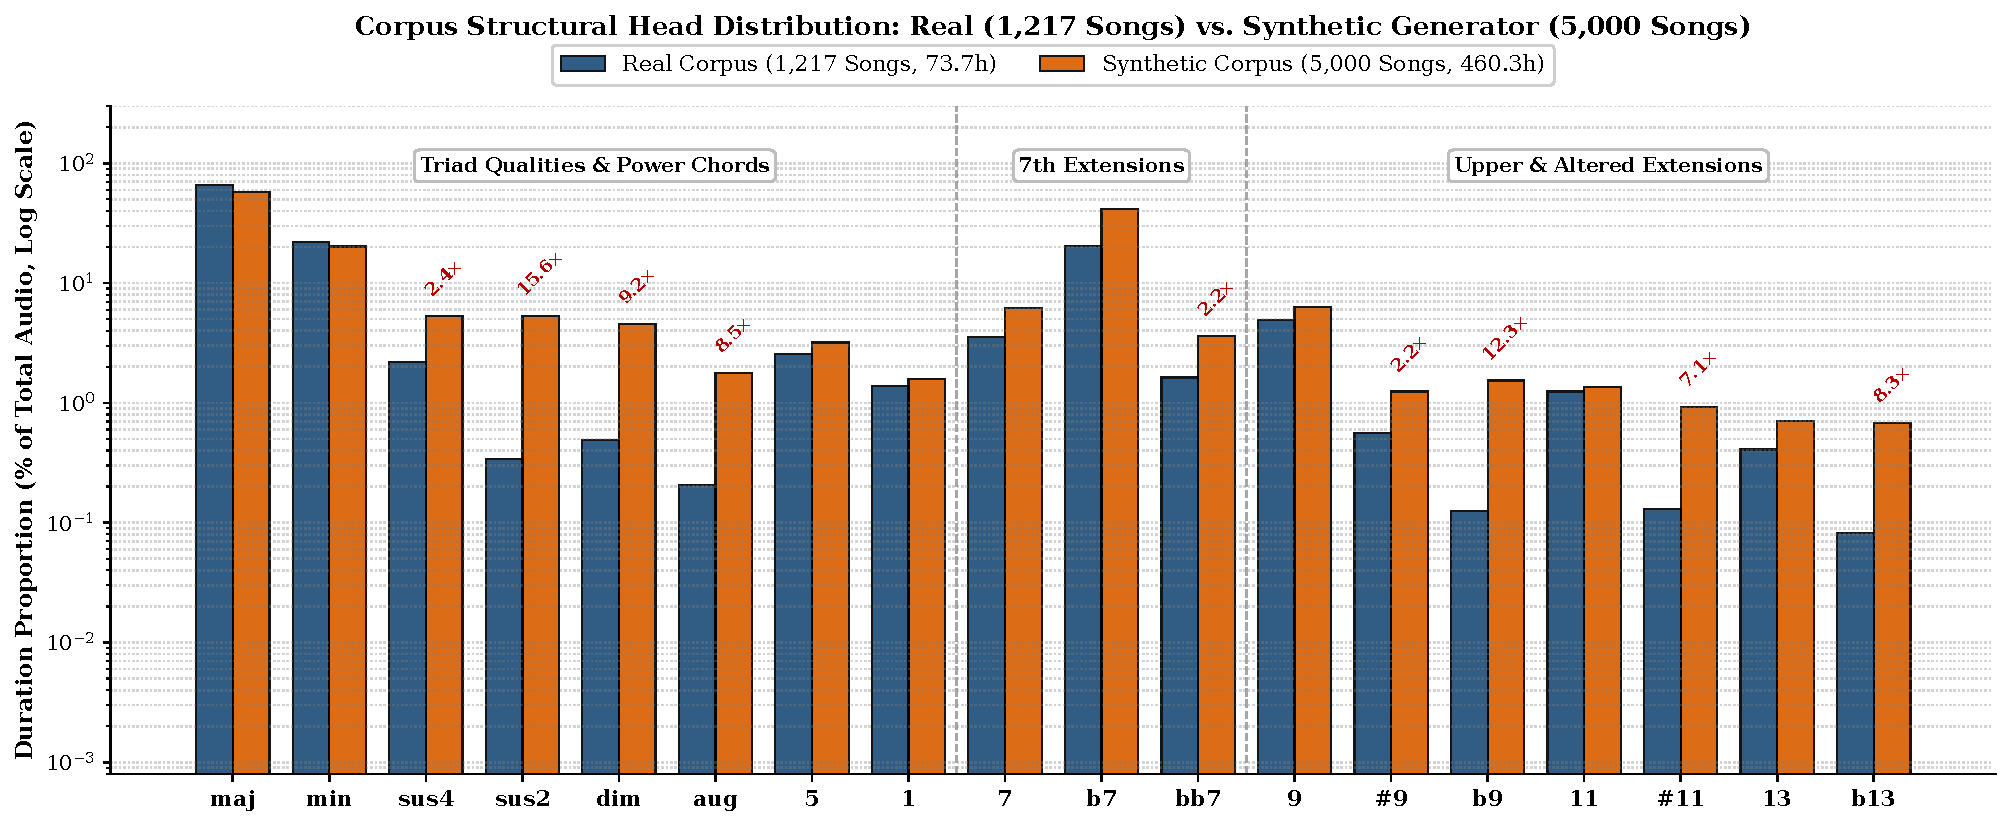
\includegraphics[width=0.74\textwidth]{figures/fig1_chord_distribution.pdf}
  \vspace{-7pt}
  \caption{Log-scale duration shares across 18 chord and extension classes in the $1{,}217$-song real benchmark ($73.7\,\text{h}$) versus our $5{,}000$-song synthetic corpus ($460.3\,\text{h}$, excluding \texttt{N}). Major ($65.75\%$) and minor ($22.16\%$) triads occupy $87.91\%$ of real audio, leaving a steep Zipfian tail; quota scheduling expands rare triads ({\small\texttt{sus2}}: $0.34\% \!\to\! 5.31\%$, $15.6\times$; {\small\texttt{dim}}: $9.2\times$; {\small\texttt{aug}}: $8.5\times$; {\small\texttt{sus4}}: $2.4\times$) and upper extensions ({\small\texttt{b9}}: $12.3\times$; {\small\texttt{b13}}: $8.3\times$; {\small\texttt{\#11}}: $7.1\times$; {\small\texttt{\#9}}: $2.2\times$).}
  \label{fig:chord_dist}
  \vspace{-5pt}
\vspace{-2mm}
\end{figure*}

\subsection{Distribution-Shifted Harmonic Sampling}\label{subsec:harmonic_sampling}

Whereas AAM~\cite{ostermann2023aam} renders $3{,}000$ tracks from random diatonic triads ($\text{I}$--$\text{vi}$), omitting $\text{vii}^\circ$, suspended/augmented triads, and $7\text{th}$--$13\text{th}$ extensions~\cite{majchrzak2026training}, we design {\small\texttt{target\_corpus\_gen.py}} as a distributional intervention over $5{,}000$ tracks ($3{,}250$ pop/rock, $r_{\text{pop}} = 0.65$; $1{,}750$ jazz, $0.35$; $500{,}000$ events, $100$/track) along transitions extracted via ChoCo~\cite{deberardinis2023choco} from McGill Billboard~\cite{burgoyne2011expert} and Isophonics~\cite{mauch2009omras} ($1{,}114$ songs, $139{,}078$ events) plus the Weimar Jazz Database~\cite{pfleiderer2017inside} and iReal Pro\footnote{\url{https://www.irealpro.com}} ($2{,}477$ charts, $161{,}022$ events).

We parameterize each event $C_t$ by extending the 6-head space of Jiang et al.~\cite{jiang2019large} and ChordFormer~\cite{akram2026chordformer}: whereas both works restrict Head~0 to $6$ triad qualities ($73$ classes, $100$ logits)---omitting incomplete triads {\small\texttt{5}} and {\small\texttt{1}} in training and collapsing them into {\small\texttt{maj}} at evaluation---synthesizing standalone {\small\texttt{5}} and {\small\texttt{1}} exemplars allows us to expand Head~0 to $8$ qualities $q_t \in \{\text{\small\texttt{maj}}, \text{\small\texttt{min}}, \text{\small\texttt{sus4}}, \text{\small\texttt{sus2}}, \text{\small\texttt{dim}}, \text{\small\texttt{aug}}, \text{\small\texttt{5}}, \text{\small\texttt{1}}\}$ across roots $r_t \in \mathbb{Z}_{12}$ to form $S_t = (r_t, q_t)$ ($\hat{\mathbf{z}}_{0,t} \in \mathbb{R}^{97}$ with {\small\texttt{N}}); bass $b_t = (r_t + \Delta_{\text{bass},t}) \bmod 12$ for $\Delta_{\text{bass},t} \in \mathbb{Z}_{12}$ ($\hat{\mathbf{z}}_{1,t} \in \mathbb{R}^{13}$); and $\mathbf{E}_t = (e_{7,t}, e_{9,t}, e_{11,t}, e_{13,t})$ spans $\{\text{\small\texttt{N}}, \text{\small\texttt{7}}, \text{\small\texttt{b7}}, \text{\small\texttt{bb7}}\}$ ($\hat{\mathbf{z}}_{2,t} \in \mathbb{R}^4$, mapping {\small\texttt{dim7}} and, following ChordFormer~\cite{akram2026chordformer}, {\small\texttt{maj6}}/{\small\texttt{min6}} to {\small\texttt{bb7}}; Jiang et al.~\cite{jiang2019large} instead map the sixth to the 13th head), $\{\text{\small\texttt{N}}, \text{\small\texttt{9}}, \text{\small\texttt{\#9}}, \text{\small\texttt{b9}}\}$ ($\hat{\mathbf{z}}_{3,t} \in \mathbb{R}^4$), $\{\text{\small\texttt{N}}, \text{\small\texttt{11}}, \text{\small\texttt{\#11}}\}$ ($\hat{\mathbf{z}}_{4,t} \in \mathbb{R}^3$), and $\{\text{\small\texttt{N}}, \text{\small\texttt{13}}, \text{\small\texttt{b13}}\}$ ($\hat{\mathbf{z}}_{5,t} \in \mathbb{R}^3$), totaling $124$ logits. Per song ($4/4$ meter), we sample tonic $k \sim U_{\mathbb{Z}}(0, 11)$ ($S_1 \in \{\text{\small\texttt{0\_major}}, \text{\small\texttt{0\_minor}}\}$), $\text{BPM} \sim U_{\mathbb{Z}}(60, 180)$, and durations $d_t \in \{8, 6, 4, 3, 2, 1.5, 1\}$ ({\small\texttt{ww}}--{\small\texttt{q}}) with pop/rock weights $(.02, .03, .60, .05, .20, .05, .05)$ and jazz weights $(.01, .01, .30, .08, .40, .05, .15)$ ($\Delta t_{\text{sec}} = 60 d_t / \text{BPM}$).

In {\small\texttt{chord\_gen.py}}, sequence transitions factorize as:
\begin{equation}\label{eq:chord_factorization}
  \begin{split}
    P(C_t \!\mid\! C_{t-1}, C_{t-2}) &= P(S_t \!\mid\! S_{t-1}, S_{t-2})\,P(b_t \!\mid\! r_t, b_{t-1}) \\
    &\quad \cdot P(\mathbf{E}_t \!\mid\! S_t, b_t, \mathbf{E}_{t-1}).
  \end{split}
\end{equation}
Stage~1 interpolates order-2, order-1, and unigram tables via Witten-Bell weights $\lambda_i = n_i / (n_i + D)$ ($D = 25.0$):
\begin{equation}\label{eq:wb_backoff}
  \begin{split}
    P_{\text{final}}(S_t) &= \lambda_2 P_{\text{L2}}(S_t \!\mid\! S_{t-1}, S_{t-2}) + (1 - \lambda_2) \\
    &\quad \cdot \bigl[\lambda_1 P_{\text{L1}}(S_t \!\mid\! S_{t-1}) + (1 - \lambda_1) P_{\text{L0}}(S_t)\bigr],
  \end{split}
\end{equation}
using tempered $P_{\text{L1}} \propto P_{\text{raw}}^{1/\tau_1}$ ($\tau_{1,\text{pop}} = 2.2$, $\tau_{1,\text{jazz}} = 2.0$), floor $(1 - \epsilon) P_{\text{final}} + \epsilon P_{\text{L0}}$ ($\epsilon = 0.02$), and repeat discount $\delta = 0.20$ on $S_t = S_{t-1}$. Stage~2 applies order-1 bass backoff ($D = 25.0$), adds whole/half-note slash inversions at $p_{\text{inv}} = 0.10$ ($0.60$ $3\text{rd}$, $0.40$ $5\text{th}$), and slices sub-measure passing bass motion. Stage~3 walks a 4-slot prefix trie across state Trie~A ($N \ge 200$), triad Trie~B ($N \ge 500$), and genre Trie~C with $(b_t, \mathbf{E}_{t-1})$ backoff, merges enharmonic collisions ({\small\texttt{bb7+13}}, {\small\texttt{sus4+11}}, {\small\texttt{sus2+9}}, {\small\texttt{dim+\#11}}, {\small\texttt{aug+b13}}), and injects $p_{\text{NC}} = 0.01$ silence ({\small\texttt{N}}) solely on unextended root-position {\small\texttt{maj}}/{\small\texttt{min}} triads.

We partition tracks ($r_{\text{nat}} = 0.50$) into $2{,}500$ natural and $2{,}500$ targeted songs. For class $k$ with count $c_k$, quota $Q_k$ ($S_{\text{triad}} = 3.0\times$ on rare triads), event budget $N_{\text{ev}}$, and buffer $B \in \{50, 5{,}000\}$, due positions satisfy:
\begin{equation}\label{eq:quota_due}
  \text{pos}_{\text{due}}(k) = \left\lfloor \frac{(c_k + 1) N_{\text{ev}} + (Q_k + B) - 1}{Q_k + B} \right\rfloor,
\end{equation}
spaced by $\Delta_{\text{pos}} \ge 2$ along attested 1- or 2-step edges weighted by $P_{\text{dist1}}(s) C_{\text{local}}(s) / (1 + \text{RootCount}(s))$ ($3.38\times$--$95.8\times$ empirical upweighting). Versus the $1{,}217$-song corpus (Figure~\ref{fig:chord_dist}), duration shares rise across {\small\texttt{sus2}} ($0.34\% \!\to\! 5.31\%$, $15.55\times$), {\small\texttt{dim}} ($0.49\% \!\to\! 4.53\%$, $9.20\times$), {\small\texttt{aug}} ($0.21\% \!\to\! 1.77\%$, $8.50\times$), {\small\texttt{sus4}} ($2.21\% \!\to\! 5.28\%$, $2.40\times$), {\small\texttt{b7}} ($20.30\% \!\to\! 41.55\%$), {\small\texttt{bb7}} ($1.62\% \!\to\! 3.61\%$), {\small\texttt{b9}} ($0.13\% \!\to\! 1.54\%$, $12.28\times$), {\small\texttt{b13}} ($0.08\% \!\to\! 0.68\%$, $8.34\times$), {\small\texttt{\#11}} ($0.13\% \!\to\! 0.92\%$, $7.12\times$), {\small\texttt{\#9}} ($0.56\% \!\to\! 1.25\%$, $2.22\times$), {\small\texttt{9}} ($4.90\% \!\to\! 6.27\%$), {\small\texttt{13}} ($0.41\% \!\to\! 0.71\%$), and {\small\texttt{11}} ($1.25\% \!\to\! 1.36\%$).

\subsection{Symbolic Realization and Voicing Heuristics}\label{subsec:voicing}

Adapting AAM's four-stem JFugue paradigm~\cite{ostermann2023aam} ({\small\texttt{render.py}}), we map $4/4$ 16th-note grids ($4$ slots/beat) across: {\small\texttt{V0}} ($70\%$ pads, $30\%$ arpeggios), {\small\texttt{V1}} (bass in $[28, 55]$, $\text{E}_1$--$\text{G}_3$, playing roots, inversions, walking/passing lines, and $p_{\text{jump}} = 0.20$ octave leaps), {\small\texttt{V2}} (beam-search or random-walk melody masking $\{3, 4\}$ on {\small\texttt{sus2}}/{\small\texttt{sus4}}/{\small\texttt{1}} and restricting {\small\texttt{5}} to $\{0, 5, 7, 10\}$), and {\small\texttt{V9}} (Channel~10 drums).

Six policies parameterize {\small\texttt{V0}} MIDI bounds $[w_{\text{lo}}, w_{\text{hi}}]$ and voice limits $[V_{\text{min}}, V_{\text{max}}]$~\cite{tymoczko2011geometry}: {\small\texttt{pop-piano}} ($[43, 88]$, $[3, 7]$), {\small\texttt{pop-guitar}} ($[40, 76]$, $[3, 6]$), {\small\texttt{pop-synth}} ($[36, 96]$, $[3, 8]$), {\small\texttt{jazz-piano}} ($[48, 84]$, $[3, 6]$), {\small\texttt{jazz-guitar}} ($[45, 79]$, $[3, 5]$), and {\small\texttt{jazz-synth}} ($[40, 91]$, $[3, 7]$), with guitar policies enforcing $\le 4$-fret spans (cap $\le 12/15$) and barr\'e/drop shapes to prevent seventh-chord collapse across fretboard acoustics~\cite{nadar2019towards}. Unlike shell voicers that drop extensions, {\small\texttt{voicing/select.py}} enforces acoustic faithfulness: (1) $100\%$ of $7\text{th}$--$13\text{th}$ extensions sound in piano/synth policies, while guitar policies allow fallback only below Step~8 of an 8-level ladder at $+60.0 N_{\text{dropped}}$ penalty ($< 0.5\%$ drop rate); (2) the Distinguishing Chord Tone ($13\text{th} > 11\text{th} > 9\text{th} > 7\text{th} > 3\text{rd} > 5\text{th}$) avoids upper-root masking via top, isolated, or octave exposure; (3) $3\text{rds}$ never drop and $5\text{ths}$ omit ($p_{\text{omit\_5th}} \in [0.10, 0.70]$) only on {\small\texttt{maj}}/{\small\texttt{min}}; and (4) {\small\texttt{V0}} root omission ($p_{\text{omit\_root}} \in [0.02, 0.75]$) requires active {\small\texttt{V1}} bass. After low-interval and cluster pruning, we sample voicings via $P(c) \propto \exp(-(C(c) - \min C)/\tau_{\text{voic}})$ ($\tau_{\text{voic}} \in [2.2, 6.0]$) under:
\begin{equation}\label{eq:voicing_cost}
  \begin{split}
    C(c) &= w_{\text{vl}} d_{\text{vl}}(p_{\text{prev}}, p_c) - B_{\text{plr}} \\
    &\quad - 0.5 \min(|p_{\text{prev}} \cap p_c|, 3) + C_{\text{reg}}(c),
  \end{split}
\end{equation}
combining minimal voice-leading distance $d_{\text{vl}}$~\cite{tymoczko2006geometry,eitel2024perception} (solved via Hungarian assignment; $w_{\text{vl}} \in [0.5, 1.6]$, unmatched penalty $[1.2, 2.5]$), Neo-Riemannian $\text{P}/\text{L}/\text{R}$ bonus $B_{\text{plr}} \in [0.4, 3.0]$~\cite{cohn1998introduction,douthett1998parsimonious}, and spacing/drift cost $C_{\text{reg}}$. Five arpeggio profiles (gate $0.65$--$1.75$, velocity $78$--$96$) and {\small\texttt{HumanizedMidiRenderer.java}} prevent block-onset overfitting via $\sigma_t = 15.0\,\text{ms}$ jitter, pocket offsets ($0, +8, -4, -6, +2\,\text{ms}$ on pads, {\small\texttt{V1}}, {\small\texttt{V2}}, arpeggios, {\small\texttt{V9}}), $7.0\,\text{ms}$/string strums (GM~$24$--$31$), CC64 sustain (GM~$0$--$7$), and Gaussian velocity noise ($\sigma_v = 8.0$ harmonic; $\sigma_v = 4.0$ atop drum hits $\mathcal{N}(100, 8^2)$ kick/snare/crash, $\mathcal{N}(65, 8^2)$ ghost snare, $\mathcal{N}(80, 12^2)$ hi-hat/ride).

\subsection{Synthesis and Random-Mix Augmentation}\label{subsec:random_mix}

We synthesize stems via FluidSynth at $f_s = 22{,}050\,\text{Hz}$ ($16$-bit FLAC), rotating across four GM {\small\texttt{.sf2}} banks: {\small\texttt{FluidR3\_GM}} ($141\,\text{MB}$), {\small\texttt{MuseScore\_\allowbreak General\_\allowbreak Full}} ($468\,\text{MB}$), {\small\texttt{GeneralUser\_\allowbreak GS}} ($31\,\text{MB}$), and {\small\texttt{TimGM6mb}} ($5.7\,\text{MB}$). GM pools span $40$ {\small\texttt{V0}} patches ($16$ keyboard/organ/mallet, $12$ guitar/plucked, $12$ synth/pad), $13$ weighted {\small\texttt{V1}} bass patches (GM~$33, 34, 32, 35$ weighted $35, 25, 20, 15$), $18$ {\small\texttt{V2}} lead patches ($\ge 25\%$ vocal formants GM~$52$--$54$ in pop/rock), and randomized drum kits ($p = 0.60$ crash).

To mitigate acoustic overfitting, we mix stems via {\small\texttt{project\_\allowbreak condition\_\allowbreak corpus.py}} using Bernoulli dropout on {\small\texttt{V2}} and {\small\texttt{V9}} ($P = 0.70$ each: $49\%$ four-stem, $21\%$ {\small\texttt{cbm}}, $21\%$ {\small\texttt{cbp}}, $9\%$ {\small\texttt{cb}}) and perturb nominal gains $(0.0, +1.0, -1.0, -1.5)\,\text{dB}$ by $\Delta G_{\text{V0}}, \Delta G_{\text{V1}} \sim U(-3, +3)\,\text{dB}$, $\Delta G_{\text{V2}} \sim U(-3, +4)\,\text{dB}$, and $\Delta G_{\text{V9}} \sim U(-4, +4)\,\text{dB}$. FFmpeg applies {\small\texttt{V1}} saturation ($x - 0.05x^3$), $120\,\text{Hz}$ shelf ($+2.0\,\text{dB}$), and $3.5\,\text{kHz}$ low-pass; {\small\texttt{V0}} power-chord overdrive and cabinet EQ ($-3.0, +2.5, -6.0\,\text{dB}$ at $0.1, 0.25, 4.5\,\text{kHz}$); stereo panning ($60/40$ {\small\texttt{V0}}, $50/50$ {\small\texttt{V2}}, $40/60$ {\small\texttt{V9}}); split-band room convolution ($1.2/0.8/0.4\,\text{s}$, $82\%/18\%$ dry/wet, $150\,\text{Hz}$ wet high-pass); detuning $\Delta f_{\text{cents}} \sim U(-25, +25)\,\text{cents}$; $\pm U(1.5, 3.0)\,\text{dB}$ tilt at $1.5\,\text{kHz}$; console saturation ($x - 0.1x^3$); bus compression ($20/150\,\text{ms}$); and $-18.0\,\text{LUFS}$ normalization ($-1.0\,\text{dBTP}$ ceiling). This forces the Conformer~\cite{gulati2020conformer,akram2026chordformer} to extract timbre-invariant pitch-class profiles across polyphonic masking and detuned CQT bins. Across all $5{,}000$ tracks ($460.3\,\text{h}$), {\small\texttt{start\_\allowbreak padding\_\allowbreak frames=0}} anchors sample~$0$ to $t = 0.000\,\text{s}$, exporting frame-exact Harte {\small\texttt{.lab}} labels~\cite{harte2005symbolic} free of human annotation subjectivity~\cite{koops2019annotator}.
